\chapter{Results}
\section{Users}
  In total, 15 people participated in the user study.
  They were recruited from MIT students,
  via dorm and living group mailing lists.

  All of the 15 people participated in the opening and closing interviews.
  However, only 8 of them participated in the Android portion of the study.
  The reasons for this will be discussed in the Section \ref{sec:Android}.

  The participants were compensated for their degree of participation,
  and the compensation structure is outlined in Table \ref{table:compensation}.
  in Appendix A.

\section{Opening Questionnaire Results}
  The results from the opening questionnaire help to characterize the group's
  general thoughts on the subject of stress and support.
  
  Part of the survey included questions, scored on a Likert Scale,
  addressing to what degree they reach out to friends or family when troubled,
  and to what degree they feel supported by friends and family.
  The results are shown in Figure \ref{fig:likert}.

    \begin{figure}
    \centering
    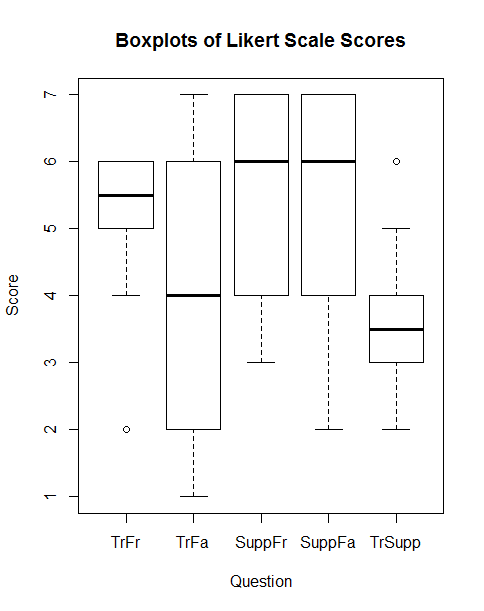
\includegraphics[width=0.6\textwidth]{likert.png}
    \caption[Likert Scale Box Plots]{
      Results of Likert scale styled questions on the opening questionnaire.
      TrFa and TrFa asked whether participants want to talk to
      Friends or Family when Troubled.
      SuppFa and SuppFa asked whether participants felt supported by
      Friends or Family.
      TrSupp asked if they reached out, in general, when troubled.
    }
    \label{fig:likert}
    \end{figure}

  Also in the opening questionnaire, we administered a Perceived Stress Scale.
  The results, shown in a histogram in Figure \ref{fig:perceived_stress},
  show that in general, the users in this study had relatively low
  self-reported stress.

    \begin{figure}
    \centering
    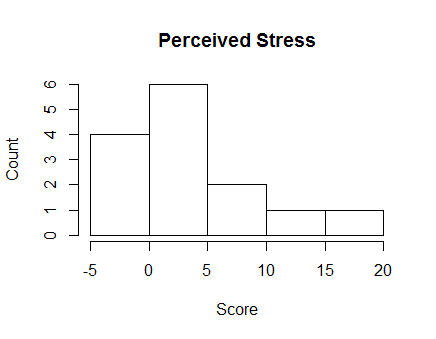
\includegraphics[width=0.6\textwidth]{perceived_stress.png}
    \caption[Perceived Stress]{
      Distribution of Perceived Stress scores amongst the 15 participants.
    }
    \label{fig:perceived_stress}
    \end{figure}

\section{Opening Interview: Script Based Results}
  The opening interview, as mentioned in Section \ref{sec:opening_int},
  followed a script, so I'll briefly outline some of the
  prominent results from the 5 sections.

  \subsection{Support-Interest}
  Because the participants' situations were so different,
  the degree to which they wanted or needed social support were very different as well.
  I assessed their general degree of need and interest in reaching out,
  what I call support-interest, during the interview.
  I define support-interest as the trait of consistently having a desire
  and making efforts to
  connect on an emotional and empathetic level with loved ones.
  Based on the nature of their support network
  and how they choose to interact with the members in it,
  it is relatively straightforward to characterize the interviewee's
  current level of support-interest.
  From the interviewees descriptions, support-interest isn't an inherent trait,
  and is instead also dependent upon the current situation of the interviewee.

  Interviewees on the low support-interest end
  have a preference for keeping their concerns to themselves.
  Two interviewees seemed especially independent,
  expressing a desire for and general pattern of dealing with things alone,
  without much external input.
  They were by no means not social.
  Both reported having plenty of friends that they interacted with regularly,
  but they chose to keep them at a greater distance when it came to things
  they were particularly sensitive about.
  When asked
  about how they discuss serious subjects with those closest to them,
  they tend to express a lack of interest.
  A quote from one of them
  helps to express the sentiment:
  \begin{itemize}
  \item
  \textit{
  ``[These thoughts are] my personal complications.
  I usually don't share that much with people because
  I'm not comfortable with them knowing me too well.
  I prefer to keep a personal boundary."
  }
  - Participant 1847, on her thoughts about keeping her privacy,
  \end{itemize}

  On the high support-interest end, there was a lot of variability.
  High support-interest people included my married interviewees, who notably,
  married within the last 5 years or so,
  and expressed being very open with their spouses, sharing everything.
  They also included a participant very active in her church community,
  and other individuals close with their parents or significant others.
  These participants expressed spending a lot of time invested in
  sharing feelings and struggles.
  Quotes associated with them included:
  \begin{itemize}
  \item \textit{
  ``She was the first person that I felt like I could talk freely with.
  We can talk about anything and everything.
  She asks questions that really pin at trying to figure out
  where emotions are coming from, what's really bothering me at a certain time.
  Just the fact that she lets me talk freely and with understanding
  makes me more comfortable."
  }
  - Participant 8594, about her mentor figure.
  \item \textit{
  ``I talk most to my mom... I try to tell my mom everything.
  She's not pushy, but she won't let me not tell her things.
  She'll ask `And then what did the the doctor say? And then?
  What's this medicine? I need to look it up!'
  [So] then I tell her everything, because she worries."
  }
  - Participant 1496, about her mother.
  \item  \textit{
  ``We're on GChat a lot.
  We chat throughout the day.
  I know how she's feeling with about a 15 minute resolution."
  }
  - Participant 3792, about his girlfriend.
  \item \textit{
  ``I have a really honest relationship with [boyfriend name].
  He'll be the first one to check in after a medical appointment,
  so is most aware...
  Rather than him trying to make sense of it,
  it makes more sense for him to just be supportive and be there.
  ... If I say anything negative, he'll jump on it.
  If I'm feeling down on myself,
  just him kinda being, `Hey, you're doing the best you can.'
  ... Sometimes I'm in the place to hear it."
  }
  - Participant 4416, about her boyfriend.
  \item \textit{
  ``I have a group of two women.. we call ourselves accountability partners.
  We meet up, like, every week.
  The idea of keeping each other accountable is
  [about] committing to listen to one another, encourage one another,
  and challenge one another to live a life of faith."
  }
  - Participant 5397, about her certain members of her church community.
  \end{itemize}

  \subsection{Choosing People and Choosing Topics}
  On discussing the support network of the interviewees,
  they tended to have a certain group of people that they turned to for
  general day-to-day support.
  These people could be family, or family-like people, as well as friends,
  but most times, participants had a strong preference towards one or the other.

  In most cases, the interviewee chose to discuss serious subjects ---
  about things that were really on their minds ---
  with only friends or only family,
  and chose to discuss only mundane, less serious topics with the other.
  For example, Participant 1010, talking about her parents,
  expressed a common sentiment.
  \textit{
  ``We only talk about mundane things...
  things not directly related to life."
  }

  \subsection{Serious Situation}
  Although the call for participant recruitment called for participants
  dealing with some serious situation in their lives,
  whether mourning or illness or other unusual difficulty of transition,
  the severity of the participants' situations varied.

  On the lighter end of the spectrum included six participants who were
  dealing with regular academic and career pressures.
  On the heavier end,
  three participants were dealing with very serious chronic illnesses,
  another was bereaved,
  and others were battling other forms of daunting transitions and trials.

  \subsection{Meeting Needs}
  Luckily, all of my participants who wanted support had people
  who could provide it.
  However, as anticipated by other research \cite{skeels10},
  when the needs grew, it became harder for some of my participants to get
  what they needed.

  Participant 9541 expressed a general sentiment about discussing tough topics:
  \textit{
  ``Feeling like you need it and actually reaching out are two different things.
  It's a lot harder to say `I'm struggling with whatever's going on.'"
  } and Participant 5397 described a high learning curve
  \textit{
  ``Two years ago.
  Actually, even a year ago, I was not very good about reaching out to people.
  It takes a lot of energy to reach out to people and explain what's going on.
  [We thought]
  `If these people are really my friends, they should be reaching out to me,'
  but actually, if they don't know, they don't know.
  Nowadays, there's a group of people we'll email or call.
  Maybe we should be asking a few people, specifically, to be on-call."
  }

  \subsection{Technology}
  On technology,
  my participants tended to be technically savvy.
  This is likely due to the age range of the participants,
  the youngest of which was 18, and the oldest 30.
  Consistent with previous research,
  they used a complex range of technologies to connect
  with friends and family near and at distance,
  for a range of complicated reasons.

  More convenient forms of communication,
  such as text or other forms of instance message,
  were used frequently for casual things such as keeping in touch,
  and other modes of communication, such as video, phone, or in person meetings,
  were used for more serious topics.
  The exception to this was email,
  which despite being digital and text based, 
  afforded a level of thoughtfulness that participants
  felt were especially valuable in a different way.
  One participant found emails the best medium for reconnecting
  with distant friends on the nature and current condition of her
  chronic illness,
  and another participant who had depressive episodes found that
  email communications fell better into her comfort zone during the dark times.

\section{Opening Interview: Other Trends}
  The trends addressed by the script of the opening interview touched on
  some important topics, but the most interesting results
  were other patterns and phenomena
  that were not anticipated by the script.

  \subsection{Direction of Awareness}
  In many cases, there was a clear directionality to the type of awareness
  information shared.
  One recurrent example was with parents,
  when the daughter or son tends to report a lot to the parent,
  and the parent reports relatively little in return.
  Other relationships, such as between siblings or friends,
  can also be very directional,
  with one party in the habit of disclosing more to the other.
  for example, Participant 1010 explained her relationships:
  \textit{
  ``With some of my friends, I like to know what they're doing.
  I kinda mother them.
  I like to make sure they're doing okay."
  }

  \subsection{Extreme Information Withholding}
  Another phenomenon that became apparent with interviews is that
  many, even normally trusting, close relationships,
  can incorporate extreme instances of information withholding.
  One relatively whimsical example was brought up
  when the topic of awareness and updates from family was brought up.
  \textit{
    ``
    They don't tell me anything. No.
    They feel like I should focus on me.
    Even when my dog passed away, they didn't tell me for an entire month.
    They didn't want me to be upset.
    I just noticed the dog wasn't there, and they never straight up told me."
  } - Participant 2928

  It's important to note that the story is one instance of a general
  trend of not sharing bad news.
  This can be as simple as preferring to look on the bright side:
  \textit{
  ``I try to look on the bright side.
  For example, my Facebook page used to be full of sad things.
  I decided not to do that anymore."
  } - Participant 3792
  or \textit{
  ``[My struggles are] not really fun to talk about.
  Most people already have enough on their plate"
  }
  - Participant 9451
  
  This can also be taken to the extreme.
  One specific example from my participants involved
  completely not telling family members about a serious issue,
  while maintaining communications otherwise.

  \subsection{Changes in Support Structure}
  Lastly, closely related to the extreme information withholding,
  there are many situations in our lives that result in
  drastic changes in the nature of our support structure.
  As mentioned in Section \ref{sec:intro},
  death can be the most tragic cause of such a change.
  When the person who passed away had a pivotal role in the support
  structure of another, it can be even harder to cope with
  the difficult period of mourning.
  Though this was true for a participant who was bereaved,
  the drastic changes that other interviewees described usually involved
  a falling out of some sort.
  These falling outs could be between family members,
  significant others, or even friends,
  and completely overturn an existing network.

\section{Android}
  After the Opening Interview, participants were instructed to invite
  at least 2 people to join their group.
  Once there were 3 people in a group,
  they were given the InMind application,
  and they could begin.

  \subsection{Attrition}
    \label{sec:Android}
    Of the 15 participants, 2 could not continue the Android portion
    of the study due to timing constraints.
    5 more did not get two people in their group,
    so after two weeks,
    we decided to call them in for a closing interview.

    The closing interview, instead of asking about the experience of using
    the application, just inquired into the reasons for not recruiting friends.
    One reason for failing to recruit is that users did not have friends
    who used Android phones.
    One participant asked 5 friends and discovered all were iPhone users.
    Another was that the participants simply became too busy to interact with
    friends and ask them to be in a study with them.

  \subsection{Weekly Feedback}
  During the study,
  I asked for feedback via open ended online questionnaires,
  and offered optional in-person check-ins that 3 of participants took me up on.

  Most of the weely feedback consisted of feature requests.
  Some participants wanted to be able to change the sharing status
  of a topic after it was started.
  Others wanted to be able to post pictures onto a topic.
  A full compiled list of feature requests has been compiled in Appendix B.

  In general, the suggestions were reflective of the users' experience with other
  applications for communication, such as Google Hangouts \cite{gchat},
  Line \cite{line}, or QQ \cite{QQ},
  in that users expected to be able to send pictures, emoticons, video,
  and receive notifications for messages.

  On the other hand, one participant contrasted the slow messaging design with
  the other forms of communication and said she liked knowing that the other
  people in the group weren't being immediately contacted when she wrote messages.

\section{Data and Questions to Answer}
  Since the data set only includes 8 groups,
  it is not particularly meaningful to derive any statistical conclusions
  from them.
  However, a data set of 36 users, 70 topics, and 1043 messages
  is still useful for observing some likely trends.
  The questions that I will discuss in this section address
  permissions given to topics, the life cycle of a topic,
  user interactions over 3 weeks of usage,
  and variability between the 8 groups.

  \subsection{Permissions}
  An important question posed at the beginning of this study
  considered who topics would be shared with.
  The hypothesis was that for many serious topics,
  the privacy of the information was very important to the owner of the topic,
  so the owner would want to control who had access to it.
  In this study, of the 70 topics observed, 13 were shared with no-one,
  and were used by the owners to organize their own thoughts.
  27 topics were shared with "Everyone" within the group,
  and the remaining 30 were shared with some subset of people.
  It is safe to assume from this usage data that
  there is a desire to organize tihngs for oneself,
  and the topics that are shared are roughly evenly distributed
  between those that the owner is fairly comfortable sharing with the public,
  and those that are shared with specfic people.

  \subsection{Topic Life Cycle}
  Topics are created generally in the mornings and evenings,
  presumably before the day starts and after the day ends,
  and not when things are happening.
  The distribution of hours of creation is shown in
  Figure \ref{fig:topic_hours},
  which shows a bimodal distribution centered on waking and sleeping hours.

  \begin{figure}
  \centering
  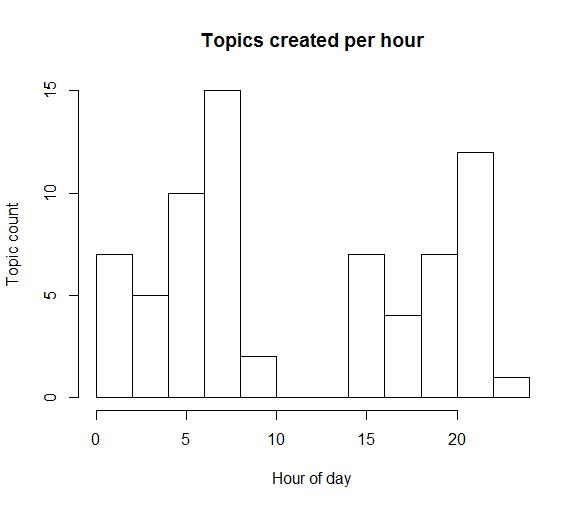
\includegraphics[width=0.6\textwidth]{topics_per_hour.jpg}
  \caption[Topics Created by Hour of Day]{
    Topics were created at varying hours of the day.
    The 70 topics shown in this bar chart appear to show
    topics being created in the morning and evenings,
    and occasionally in late evening/early morning,
    but fewer in the middle of the day, between 10:00 A.M. and 3:00 P.M.
  }
  \label{fig:topic_hours}
  \end{figure}

  After the opening interviews, we considered the types of stressors the
  interviewees faced, and postulated 2 likely types of topics.
  short lived and long lived ones.
  Short lived topics we imagined would last a few days to a week,
  and would include things like class projects,
  work deadlines, short conflicts with friends, and other temporary frustrations.
  Long lived topics we imagined would last much longer,
  and would include the more serious topics, likely the major stressor,
  and since these stressors are expected to last several months to indefinitely,
  should remain active for the duration of the 3 week study.
  This ended up remarkably accurate,
  but we had not anticipated that many topics would be created,
  and never become active.
  These "zero-day" topics were created,
  but were neither updated nor discussed after the day they were created.

  In Figure \ref{fig:topic_age}, charts show two different measures of 
  topic duration, filtered and not filtered to remove the zero-day topics.

  \begin{figure}
  \centering
    \begin{subfigure}[b]{0.4\textwidth}
      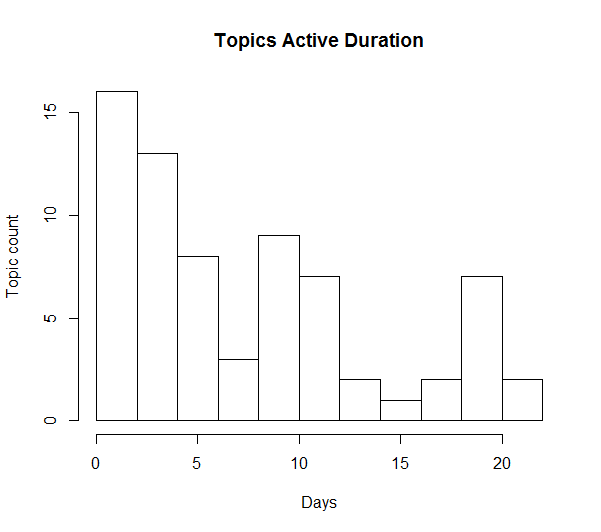
\includegraphics[width=\textwidth]{topic_days_active.png}
      \caption{Days topics were discussed after creation.}
    \end{subfigure}
    \begin{subfigure}[b]{0.4\textwidth}
      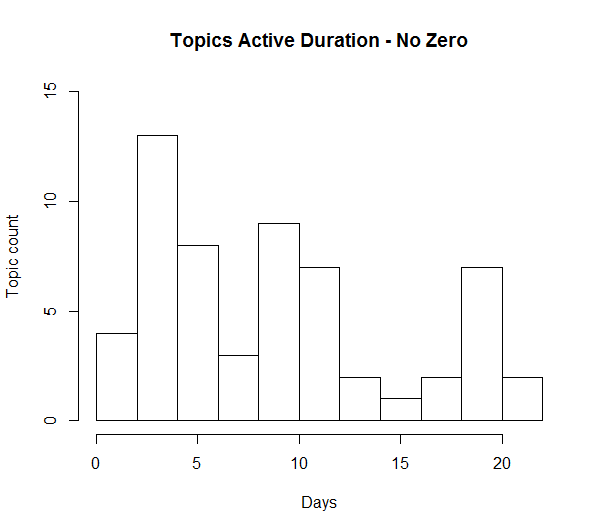
\includegraphics[width=\textwidth]{topic_days_active_nz.png}
      \caption{Days topics were discussed after creation,
        minus topics not discussed after the first day.}
    \end{subfigure} \\
    \begin{subfigure}[b]{0.4\textwidth}
      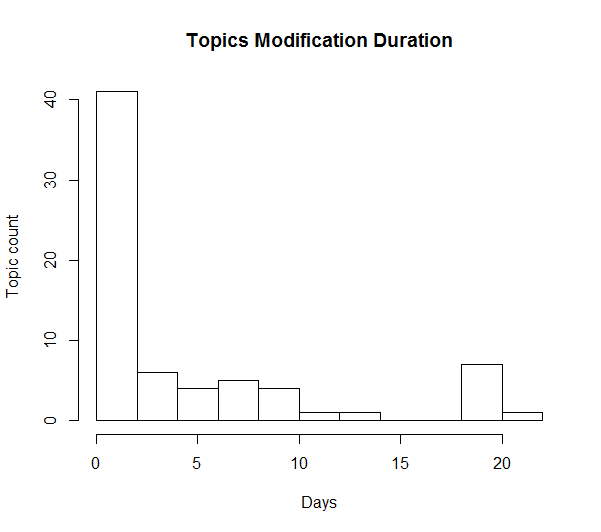
\includegraphics[width=\textwidth]{topic_days_mod.png}
      \caption{Days topics had status changed, after creation.}
    \end{subfigure}
    \begin{subfigure}[b]{0.4\textwidth}
      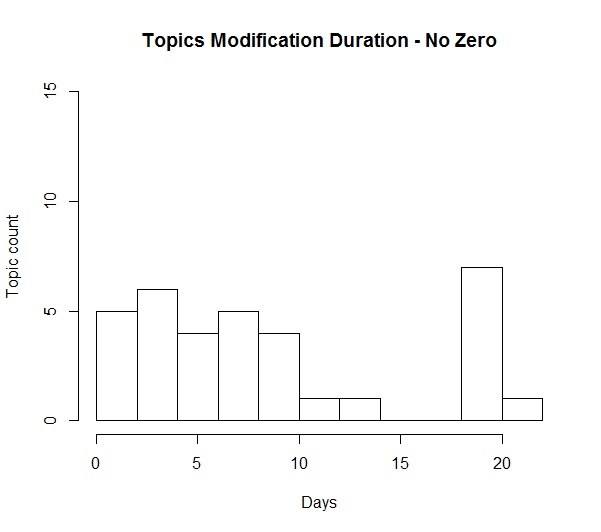
\includegraphics[width=\textwidth]{topic_days_mod_nz.png}
      \caption{Days topics had status changed, after creation, minus zeros.}
    \end{subfigure}
  \caption[Duration of Topics] {
    Topics were active for varying periods.
    Note that there are so many topics that did not have their status changed
    after the first day that the vertical scale is greater on subgraph c.}
  \label{fig:topic_age}
  \end{figure}

  \subsection{General Usage During Study}
    The number of topics created and number of messages sent changed over
    the course of the 3 weeks.
    Counts of how many of each occurred each week are summarized in
    Table \ref{table:weekly}
    On average, each group created about 5 topics the first week,
    2 topics the second week, and 1 topic the third week,
    and similarly, sent 70, 45, and 15 messages.
    This pattern is expected for both topics and messages.
    The first stage involves informing people within the
    group about both long and short term topics,
    and afterwards, only updates to long term topics,
    and creation of new short term topics are expected.
    We can reasonably postulate that the 3rd week's usage is much more likely
    to be that demonstrated by users in the long term.

    \begin{table}[h]
    \centering
    \caption{Weekly Activity}
    \label{table:compensation}
    \begin{tabular}{ l l l}
    Week & Topics Created & Messages Sent \\
    \hline
    1 & 43 & 558      \\[5pt]
    2 & 17 & 361      \\[5pt]
    3 & 10 & 124      \\[5pt]
    \hline
    Total & 70 & 1043       \\[5pt]
    \end{tabular}
    \end{table}

    How much time is spent on the app?

  \subsection{Variability Between Groups}
    The variability between groups is best explained by the
    qualitative contents of the closing interview,
    but the data gives us a preview.
    Looking at the number of messages sent within a group,
    we see that a likely typical number of messages sent within a group
    is between 30 and 100,
    but there is an outlier of more than 600 messages in one group.

    \begin{figure}
      \centering
      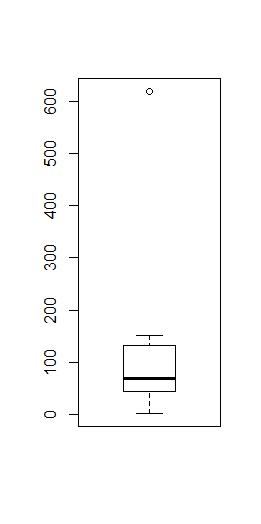
\includegraphics[width=0.3\textwidth]{messages_per_group.jpeg}
      \caption[Messages Sent by Groups]{
        The number of messages sent by each group varied between
        2 and an outlier at more than 600 messages.
      }
      \label{fig:topic_hours}
      \end{figure}

\section{Closing Interview}
  The closing interview also followed a script,
  and similarly to the opening interview, some themes quickly bubbled up from
  beyond the explicit content of the questions in the script.

  \subsection{Positive Experiences: Unique Usage Methods}
    The positive experiences were mostly reported by the people
    whose groups sent a total of more than 100 messages.
    Each of these groups found their own unique way of making the topic-based
    communication work for them.

    \subsubsection{Day-Logging}
    The group with the heaviest usage, over 600 messages in the course of 3 weeks,
    was the group surrounding Participant 5397.
    Suffering from a chronic illness,
    Participant 5397 was interested in logging her day to day activities,
    food consumption, and wellness.

    Several features of Participant 5397's habits suggest why her and her group's
    usage was so high.
    In the second week, she said, 
    \textit{``I've become more accustomed to working with InMind and had somewhat
    of a "schedule" (a very loose one) to check it before bed,
    which coincided somewhat nicely with my nightly reflection time.
    [T]he active group member has been asking me questions that might not come up
    in our typical interactions...
    This kind of daily back and forth has developed our friendship
    and made me think more."}
    This suggests a regular schedule and habit of reflection,
    and that InMind integrated smoothly with her existing habits,
    and that she got value out of having someone being on the other end,
    responding and reflecting with her.

    Further, during the closing interview, she described InMind as a convenient
    way to send logs to other people every day,
    as opposed to other forms of communication, such as email, in which she sends
    one email a week at best.

    \subsubsection{Self-Reflection}
    The second most active group was associated with Participant 8597.
    She reported early on that her friends weren't really involved in her group,
    and didn't seem to find a use for InMind, but she did.
    Participant 8594 used it for regular self reflection,
    and found personal value in using it.
    \textit{``It has helped me keep an overview of everything on my mind,
    and it let's me try to be more honest with how I assess my feelings
    on each thing."}

    \subsubsection{Activity Sharing}
    Finally, the last group that had over 100 messages was that of
    Participant 1674.
    His group's advantage was that the participants in the group were all
    more active on InMind.
    Thus, there was generally more interaction,
    and the activities were not as individually driven.
    The members of his group were in his research group,
    and they were sharing some common stressors that they could come together on.
    Further, they also were traveling together,
    and there were logistical/experience-based communications that were
    valuable for the members in the group.

  \subsection{Negative Experiences: Limitations of Study Deployment}
    \subsubsection{Sparse Interaction}
      When asked about negative experiences, 5 of the 8 participants
      described, in various ways, the disappointment associated with
      a lack of interaction from the other members within the group.
      The disappointment came specifically from instances when members of the group
      did not respond to messages sent through InMind.

      This was due to two primary reasons.
      The first reason, which applied to 1 of the 5 people,
      reflected that he expected much faster message turnover rate,
      and that for him,
      more timely responses are more useful for him, and getting a message
      several hours/a day after the incident is not helpful.
      The second reason, is related to the people in the group.
    \subsubsection{Group Membership}
      At the end of the study, when I compared the descriptions of the members
      of their actual research group with the people they reported as close
      to them during the opening interview,
      I realized that in all but 1 of the 8 groups,
      the members of the group were not people the participant would normally
      go to for support.
      The group for which the members were actually likely to be sources of support
      for the participant was that of Participant 1674.
      His group of coworkers were very close, and their interactions were
      thus the most balanced of the 8 groups.

      Besides them, every single other group was composed of
      the participant and 2 or 3 people somewhat arbitrarily drawn from
      their pool of acquaintances, based on the requirement that
      they own an Android phone.
      This is primarily a result of the study limitation imposed by requiring
      an Android device for admittance into the group,
      and it severely limited the depth of interaction possible over InMind.
      In the end, the value of the application depends on the value
      of the connections it supports.
      In one group (that of Participant 5397), it rekindled a relationship
      between the participant and an old friend,
      but in most of the groups, without existing strong ties,
      there really just wasn't much that anyone wanted to share.

  \subsection{Support Needs and Topics}
    The participants did not report any significant changes in the stressors
    in their lives,
    though the intesity of the stressors varied over the course of the 3 week study.
  
  \subsection{Meeting Needs: Dependence Upon Group Members}
    Related to the fact that membership in the group was not particularly strong,
    most of the time InMind was not used to explicitly reach out for support.
    I believe that it is due to the lack of confidence in getting a response
    from the group,
    but most consistent interactions within a group were for personal purposes,
    so instead of encouraging the actions of reaching out for help
    it seems to have encouraged self-organization and independence instead.

  \subsection{Interaction With Other Technologies}
    This topic resulted in varied results.
    Some groups (4 out of 8) brought topics from within the application to outside
    of it, via text messages, emails, or phone calls,
    and InMind functioned as an initiator for conversations.
    In many ways, this was the primary function of InMind,
    to give serious topics a place in the minds of the relevant close ties,
    and allow them to bring it up over richer communication pathways.

    For 3 out of the 8 groups, not so coincidentally the lower usage rate groups,
    topics that existed within InMind stayed within InMind,
    and never made it into the participants other interactions with their group
    members, again because they weren't particularly close with them to begin with.

